\nonstopmode
%==============================================================================
%== template for LATEX poster =================================================
%==============================================================================
%
%--A0 beamer slide-------------------------------------------------------------
\documentclass[final]{beamer}

\usepackage{graphicx}
\usepackage{xcolor}
\usepackage[orientation=portrait,size=a0,
            scale=2.2         % font scale factor
           ]{beamerposter}
           
\geometry{
  hmargin=2.5cm, % little modification of margins
}

%
\usepackage[utf8]{inputenc}
\usepackage{ragged2e}

\linespread{1.15}
%
%==The poster style============================================================
\usetheme{sharelatexback}

%==Title, date and authors of the poster=======================================
%\title
%[http://python.fossee.in, info@fossee.in, python@fossee%.in] % Conference
%{ % Poster title
%}


%\author{ % Authors
%Author One\inst{1}, Author Two\inst{2}, Author Three\inst{2,3}
%}
%\institute
%[Very Large University] % General University
%{
%\inst{1} Very Large University, Neverland
%\inst{2} Other University, Neverland
%\inst{3} Yet Another University, Neverland
%}
%\date{\today}



\begin{document}
\begin{frame}[t]
%==============================================================================
\begin{multicols}{2}
%==============================================================================
%==The poster content==========================================================
%==============================================================================

%% BACK

\section{How can you learn Python ?}
\begin{itemize}
\item \justifying {{\bf{Spoken Tutorial}} - A library of spoken
  tutorials on 'Python' is freely available, to watch, learn and
  practice for taking those initial steps and moving on. This is the
  place that helps you getting started in the world of FOSS. Learn at
  your will, any time, anywhere!  Learn Python here:
  {\color{blue}http://python.fossee.in/spoken-tutorials/}} \par

\vskip5ex

\begin{figure}
\centering
\fboxsep=0mm%padding thickness
\fboxrule=1pt%border thickness
\fcolorbox{gray}{white}{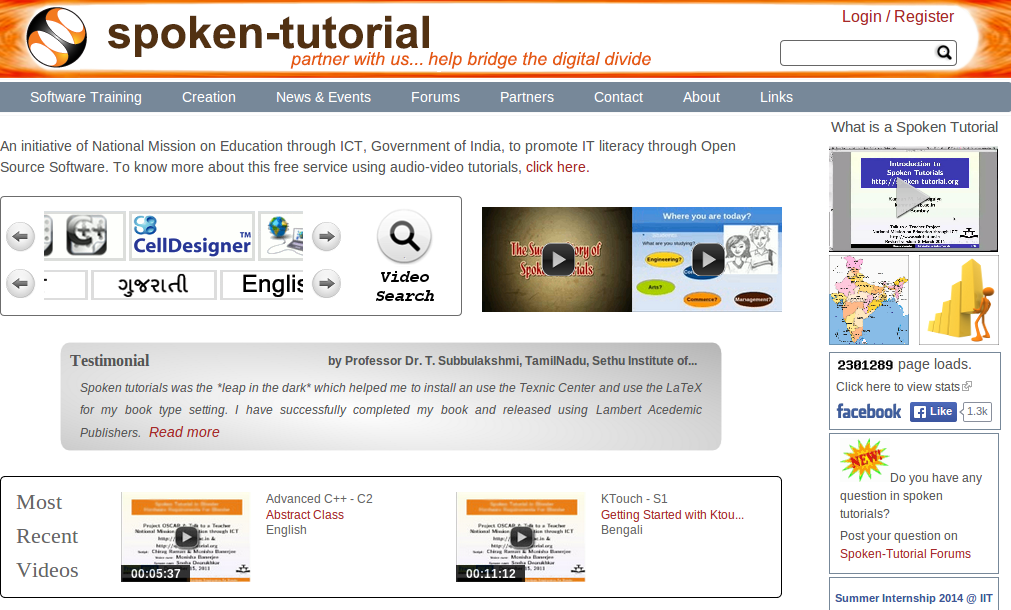
\includegraphics[width=0.9\columnwidth]{spoken-tutorial.png}}
\texttt{\small Spoken tutorial website}
%\caption{Spoken tutorial website}
\end{figure}

\vskip5ex

\item \justifying{{\bf{Textbook Companion Internship}} - Learn Python
  in a practical way by contributing to the Python Textbook Companion
  Internship. It aims to create Companions by coding solved examples
  from Standard textbooks using Python. Participate and earn
  attractive honorarium and Certificate of Internship from FOSSEE, IIT
  Bombay!  For more details, please visit - \\
  {\color{blue}http://python.fossee.in/textbook-companion-project/}}\par

\vskip5ex

\begin{figure}
\centering
\fboxsep=0mm%padding thickness
\fboxrule=1pt%border thickness
\fcolorbox{gray}{white}{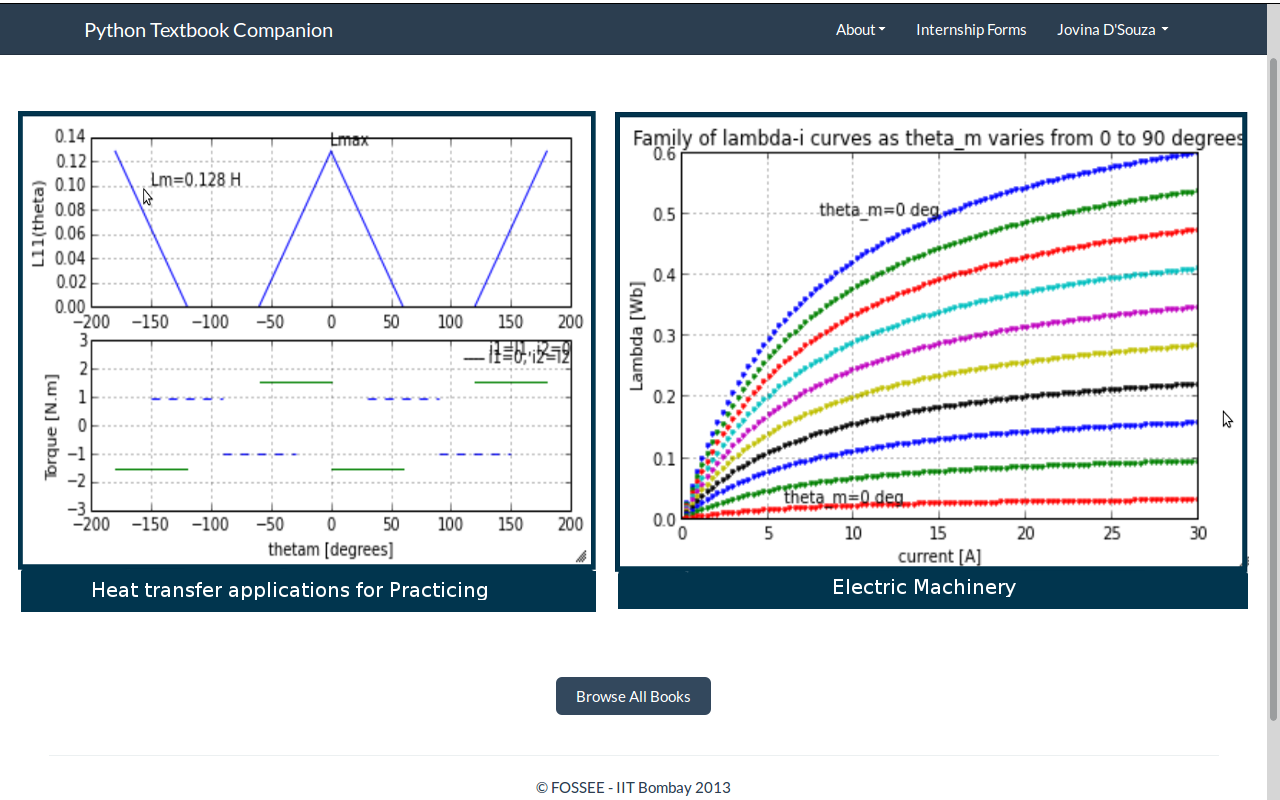
\includegraphics[width=0.9\columnwidth]{tbc.png}}
\texttt{\small Python textbook companion}
%\caption{Python textbook companion}
\end{figure}
\end{itemize}

\vskip5ex

\item {{\bf{SELF Workshops}} - Workshops on Python are conducted
  remotely by IIT Bombay. These workshops are completely free of cost
  and contain high quality material taught by experts. During these
  workshops, the participants use Spoken tutorials to work on various
  exercises and examples. Learn Python and obtain a certificate from
  IIT Bombay upon successful completion of a post-workshop test.
  Please visit, \\
  {\color{blue}http://python.fossee.in/spoken-tutorials/}}

  \vskip5ex  

\section{Contact us}
\subsection{About the project:}
\begin{center}
http://python.fossee.in/
\end{center}

\subsection{General help \& Queries:}
\begin{center}
info@fossee.in \\
python@fossee.in
\end{center}



%==============================================================================
%==End of content==============================================================
%==============================================================================
%--References------------------------------------------------------------------
%--End of references-----------------------------------------------------------

\end{multicols}

%==============================================================================
\end{frame}
\end{document}
